
\documentclass{article}
\usepackage{tikz}
\usetikzlibrary{arrows}

\begin{document}

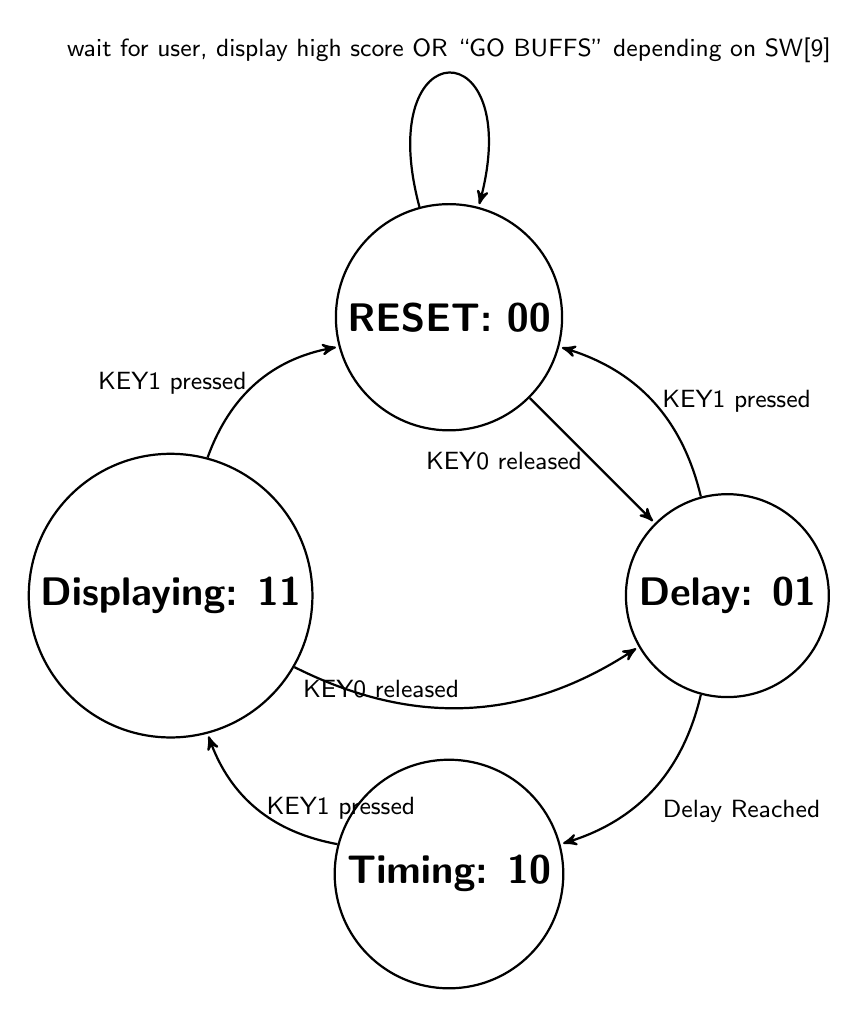
\begin{tikzpicture}[->,>=stealth',shorten >=1pt,auto,node distance=5cm,
                    thick,main node/.style={circle,draw,font=\sffamily\Large\bfseries}]

  \node[main node] (1) {RESET: 00};
  \node[main node] (2) [below left of=1] {Displaying: 11};
  \node[main node] (3) [below right of=2] {Timing: 10};
  \node[main node] (4) [below right of=1] {Delay: 01};

  \path[every node/.style={font=\sffamily\small}]
    (1) edge node [left] {KEY0 released} (4)
        edge [loop above] node {wait for user, display high score OR ``GO BUFFS" depending on SW[9]} (1)
    (2) 
            edge [bend left] node[left] {KEY1 pressed} (1)
        edge [bend right]node {KEY0 released} (4)


    (3) edge[bend left] node [right] {KEY1 pressed} (2)
    (4)	edge [bend right] node [right]{KEY1 pressed} (1)

    (4)	edge [bend left] node {Delay Reached} (3)
;
\end{tikzpicture}

\end{document}